% TEXTALLION
% http://textallion.googlecode.com
% \LaTeX template 

\documentclass[openany]{book} % openany to remove the blank pages
%\documentclass[oneside]{book}
%\documentclass{article}
%\documentclass[twoside]{article}
%\nogbitemsep ?
% book = margins are shifted
% article = no shift for margins


\usepackage[pdftex]{graphicx}
\usepackage{paralist} % needed for compact lists
\usepackage[normalem]{ulem} % needed by strike
%  %hyperref defined elsewhere
\usepackage[utf8]{inputenc}  % char encoding
\usepackage{../includes/sample_cyoa}  % user defined

\usepackage{gamebook} % [debug,draft]

%---------------- Author & Metatags ------------------------------------

\def\DOCUMENTxTITLE{La Mort Bleue} % Titre of the document
\def\PDFAUTHOR{Otto Grimwald}      % Authors
\def\PDFTITLE{\DOCUMENTxTITLE}      % copy of Titre of the document
\def\PDFSUBJECT{cyoa, steampunk} % Subjet
\def\PDFKEYWORDS{cyoa, steampunk}   % keywords, tags
\def\PDFCREATOR{Textallion, txt2tags, PdfTeX}   % Sofware which made this document
\def\PDFPRODUCER{Textallion}         % Compagny which made the software

% 

\usepackage[english,frenchb,francais]{babel}  
\usepackage[T1]{tipa}                       % additionnal fonts
\usepackage[\DEFAULTxFONTxSIZE pt]{extsizes} 
\usepackage[cm]{aeguill}                    % French guillemets
\usepackage[\SIZExOFxPAPER, \ORIENTATIONxOFxPAPER, total={\WIDTHxOFxTEXT mm,\HEIGHTxOFxTEXT mm},\GEOMETRYxADDITIONALxOPTION]{geometry}       % paper and text size
\usepackage{..//core/textallion}  % basic \LaTeX definitions for textallion

\def\MYxFONT{\rm}   % For correcting footers
\def\MYxFONTxMONO{}   % For correcting code area

%
% ------------ FONTS ---------------------------------------------------
\renewcommand{\rmdefault}{\DEFAULTxFONT} 
%



\title{The Blue Death}
\author{by Otto Grimwald}

\renewcommand{\gbturntext}{turn~to~}
\renewcommand{\gbheadtext}{\title}

\begin{document}
\begin{LARGE} \renewcommand*{\labelgbitemi}{$\bullet$} \renewcommand*{\labelgbitemii}{$\circ$} \renewcommand*{\labelgbitemiii}{$\cdot$} \renewcommand*{\labelgbitemiv}{$\diamond$}

\raggedbottom % avoid vertical jutification

\date{2013-01-29}
\maketitle
% remove first page numbering on the cover
\thispagestyle{empty}
%\setcounter{page}{0}

\clearpage

\gbheader

%\pagestyle{headings} % page numbers_
%\pagenumbering{roman} % Roman numerals
%\setcounter{page}{2}


\begin{center}\htmladdnormallink{(the\_blue\_death.jpg)}{1}\end{center} 

\hypertarget{0}{}
\pagebreak[\PAGExBREAKxPOLICY]
\textbf{\begin{center}\subsection*{\Huge{0}}\end{center}\vskip-2em}

\begin{gbitemize}
\gbitem Start the game: \textbf{\htmladdnormallink{1}{\#1}}
\end{gbitemize}

\hypertarget{1}{}
\pagebreak[\PAGExBREAKxPOLICY]
\textbf{\begin{center}\subsection*{\Huge{1}}\end{center}\vskip-2em}

I'm falling down. Not very far from the "ground", fortunately for me. Some thick, heavy ropes are softening my falling. I've probably missed my step, because I'm absent-minded most of the time now.

\begin{gbitemize}
\gbitem Stand up: \textbf{\htmladdnormallink{19}{\#19}}
\end{gbitemize}

\hypertarget{2}{}
\pagebreak[\PAGExBREAKxPOLICY]
\textbf{\begin{center}\subsection*{\Huge{2}}\end{center}\vskip-2em}

As soon as I enter the big building, some officiers catch me, for the reason of escaping a residence I was supposed to stay in, having been legally bought by Mr and Mrs Caesar.

\begin{gbitemize}
\gbitem Despite my protests, I am sent to jail: \textbf{\htmladdnormallink{48}{\#48}}
\end{gbitemize}

\hypertarget{3}{}
\pagebreak[\PAGExBREAKxPOLICY]
\textbf{\begin{center}\subsection*{\Huge{3}}\end{center}\vskip-2em}

They are a bunch of six mariners. They're just having fun after all.

\begin{gbitemize}
\gbitem But I can give them a fair correction: \textbf{\htmladdnormallink{23}{\#23}}
\gbitem Or I can crawl back to the safety of the upper deck: \textbf{\htmladdnormallink{5}{\#5}}
\end{gbitemize}

\hypertarget{4}{}
\pagebreak[\PAGExBREAKxPOLICY]
\textbf{\begin{center}\subsection*{\Huge{4}}\end{center}\vskip-2em}

I ring the bell at the door. Beatrix doesn't seem very happy to see me. She was a good friend of mine before, so I don't understand her new reluctance.

She wears a pretty, light, white and gray dress, and I sense such poetry in the air that I want to tell her about what I have in my mind.

\begin{gbitemize}
\gbitem Be rude, but direct: \textbf{\htmladdnormallink{35}{\#35}}
\gbitem Be soft, but verbose: \textbf{\htmladdnormallink{28}{\#28}}
\end{gbitemize}

\hypertarget{5}{}
\pagebreak[\PAGExBREAKxPOLICY]
\textbf{\begin{center}\subsection*{\Huge{5}}\end{center}\vskip-2em}

This deck is usually reserved to the first-class passengers. I hope some officers won't notice me or I'll be in great trouble.

I've got this job on a ship to pay my travel to the Great Continent, which had been rediscovered only a few centuries ago. Meanwhile, I've always been curious about the life there, to discover if people were like us or if their culture was far too exotic to be able to live far over there. I've also tried to learn bits of their difficult language, and forced myself to use it on a daily basis. So I moved to Iricimia, which has a similar language, and even if I still don't master it, I lived there for a while, then decided to embark on this ship.

\begin{gbitemize}
\gbitem After some time, we arrive to New Londrin Haven, and I enter the city triumphally: \textbf{\htmladdnormallink{25}{\#25}}
\gbitem But before that, I could explore the haven a bit, adding less prestige to my arrival: \textbf{\htmladdnormallink{27}{\#27}}
\end{gbitemize}

\hypertarget{6}{}
\pagebreak[\PAGExBREAKxPOLICY]
\textbf{\begin{center}\subsection*{\Huge{6}}\end{center}\vskip-2em}

We enter a snobbish tea-house, in a touristic area. We quickly get bored in this place, so I propose we search a more pleasant place to entertain ourselves.

\begin{gbitemize}
\gbitem Propose her appartment: \textbf{\htmladdnormallink{42}{\#42}}
\gbitem Propose my appartment: \textbf{\htmladdnormallink{38}{\#38}}
\gbitem Propose to get an ale in the nearby tavern: \textbf{\htmladdnormallink{7}{\#7}}
\end{gbitemize}

\hypertarget{7}{}
\pagebreak[\PAGExBREAKxPOLICY]
\textbf{\begin{center}\subsection*{\Huge{7}}\end{center}\vskip-2em}

Entering the tavern, I see some of my former comrades from the ship. Surprisingly, they are not that much hostile to my presence. We take a beer together, then an other, and I end the night dancing on the tables, to the great joys of the maids here who are clapping their graceful hands in rhythm.

I appreciate this simple life, and no longer fear the blue terror I used to feel in the past.

\begin{center} THE END \end{center} 

\hypertarget{8}{}
\pagebreak[\PAGExBREAKxPOLICY]
\textbf{\begin{center}\subsection*{\Huge{8}}\end{center}\vskip-2em}

\begin{itshape}Am I lucky today? When I get a die out of my pocket, I can be considered lucky when I cast a 5 or 6.\end{itshape}

\begin{gbitemize}
\gbitem If I'm lucky: \textbf{\htmladdnormallink{18}{\#18}}
\gbitem If I'm not lucky: \textbf{\htmladdnormallink{51}{\#51}}
\end{gbitemize}

\hypertarget{9}{}
\pagebreak[\PAGExBREAKxPOLICY]
\textbf{\begin{center}\subsection*{\Huge{9}}\end{center}\vskip-2em}

The opposition is full of nice persons, however, I can't garantee the leaders are politically clean. Some people claims they're even infiltrated by the Indigo Love Syndicate. 

\begin{itshape}Am I lucky today? When I get a die out of my pocket, I can be considered lucky when I cast a 5 or 6.\end{itshape}

\begin{gbitemize}
\gbitem If I'm lucky: \textbf{\htmladdnormallink{32}{\#32}}
\gbitem If I'm not lucky: \textbf{\htmladdnormallink{49}{\#49}}
\end{gbitemize}

\hypertarget{10}{}
\pagebreak[\PAGExBREAKxPOLICY]
\textbf{\begin{center}\subsection*{\Huge{10}}\end{center}\vskip-2em}

The docks are not a pleasant place for a delicate person like me. I get the feeling that I may become an easy prey for most of the vultures here. I notice a handsome woman waiting on the pier. Some sailors I met on the ship are calling me, while entering a tavern.

\begin{gbitemize}
\gbitem Approach the lady: \textbf{\htmladdnormallink{37}{\#37}}
\gbitem Follow my previous comrades into the tavern: \textbf{\htmladdnormallink{7}{\#7}}
\gbitem Come back home: \textbf{\htmladdnormallink{31}{\#31}}
\end{gbitemize}

\hypertarget{north}{}
\pagebreak[\PAGExBREAKxPOLICY]
\textbf{\begin{center}\subsection*{\Huge{11}}\end{center}\vskip-2em}

Impassive to the human's emotions, the ship is reaching the morning mists of the other continent. Setting my foot on the pier for the first time after three weeks of spiritual torture, I feel dizzy and completely at loss. There is a big poster on the grey wall, and an exit to the rest of the town.

\begin{gbitemize}
\gbitem Read the poster: \textbf{\htmladdnormallink{27}{\#27}}
\gbitem Exit: \textbf{\htmladdnormallink{25}{\#25}}
\end{gbitemize}

\hypertarget{12}{}
\pagebreak[\PAGExBREAKxPOLICY]
\textbf{\begin{center}\subsection*{\Huge{12}}\end{center}\vskip-2em}

Before doing a frightful jump, I notice the shadow of Beatrix arriving behind me, upset and worried about myself.

\begin{gbitemize}
\gbitem She tells me she regrets her overreaction, and propose we take a drink in a teahouse in the surroundings: \textbf{\htmladdnormallink{6}{\#6}}
\end{gbitemize}

\hypertarget{13}{}
\pagebreak[\PAGExBREAKxPOLICY]
\textbf{\begin{center}\subsection*{\Huge{13}}\end{center}\vskip-2em}

The captain, arriving a moment later, feels sorry for his men's rude behavior. Bowing deeply, he requests my opinion on the route to take. Am I dreaming? Is he insane? Or maybe it's just a sick pity.

Should we head:

\begin{gbitemize}
\gbitem North, to our original the destination, the New Continent: \textbf{\htmladdnormallink{11}{\#11}}
\gbitem South, to reach a little island he's just discovered with his telescope: \textbf{\htmladdnormallink{30}{\#30}}
\gbitem West, to explore more the vast blue Ocean: \textbf{\htmladdnormallink{43}{\#43}}
\gbitem East, back to our land of departure: \textbf{\htmladdnormallink{24}{\#24}}
\end{gbitemize}

\hypertarget{14}{}
\pagebreak[\PAGExBREAKxPOLICY]
\textbf{\begin{center}\subsection*{\Huge{14}}\end{center}\vskip-2em}

Death can be sweet, when it's so blue!

\begin{center} THE END \end{center} 

\hypertarget{15}{}
\pagebreak[\PAGExBREAKxPOLICY]
\textbf{\begin{center}\subsection*{\Huge{15}}\end{center}\vskip-2em}

The sun is high in the sky, yet I feel a chill devoring my neck and my ribs. I remember my childhood in Francimia, my games in the trees and between the rare green hills of the family's domain. Later, still in the trees, reading fantasy books lying on the red and purple carpet in my hut 8 meters above the ground. I remember my mother calling me, with her high pitched voice, to eat the "Gargouaillotte à la Pisaille", a local dish.

I suddenly feel I'm turning around.

\begin{gbitemize}
\gbitem Explore more: \textbf{\htmladdnormallink{21}{\#21}}
\gbitem Go back to the boat: \textbf{\htmladdnormallink{11}{\#11}}
\end{gbitemize}

\hypertarget{16}{}
\pagebreak[\PAGExBREAKxPOLICY]
\textbf{\begin{center}\subsection*{\Huge{16}}\end{center}\vskip-2em}

I couldn't imagine being sold as a slave would be like this. It was certainly not the marketplace we could think of, I was just conducted to a dark, moisty, cellar, where I bored to death.

\begin{gbitemize}
\gbitem A few days later, I was sold to a rich family: \textbf{\htmladdnormallink{45}{\#45}}
\end{gbitemize}

\hypertarget{17}{}
\pagebreak[\PAGExBREAKxPOLICY]
\textbf{\begin{center}\subsection*{\Huge{17}}\end{center}\vskip-2em}

I dive into the dark water. Soon I feel so alone that I stop breathing.

\begin{gbitemize}
\gbitem Drown deeper to the \textbf{\htmladdnormallink{14}{\#14}}
\end{gbitemize}

\hypertarget{18}{}
\pagebreak[\PAGExBREAKxPOLICY]
\textbf{\begin{center}\subsection*{\Huge{18}}\end{center}\vskip-2em}

The walls are now cleaner without this sick poster. 

\begin{gbitemize}
\gbitem I can continue my walk to the \textbf{\htmladdnormallink{25}{\#25}}
\end{gbitemize}

\hypertarget{19}{}
\pagebreak[\PAGExBREAKxPOLICY]
\textbf{\begin{center}\subsection*{\Huge{19}}\end{center}\vskip-2em}

I've felt depressed so many years that I can't stand it any longer. Besides, my current residence and occupation is endangering my sanity and health more and more...

\setlength{\intextsep}{3mm} \begin{wrapfigure}{l}{0\textwidth} 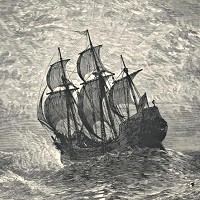
\includegraphics{../media/tbd_ship.jpg}   \end{wrapfigure} 

\htmladdnormallink{../media/tbd\_musique01.ogg}{../media/tbd\_musique01.ogg}

The blue ocean, spreading endlessly toward the all directions, is reflecting the sun like a glittering chainmail.

“Hey Francimi bastard! Come here!”, they shout.

Surrounded by those Scottani and Iricimi strangers, I don't feel at ease in this place. Their green and dark-orange helmets make me nervous. I don't really need to obey, they're just basic sailors like me. But could I bear the insults?

\begin{gbitemize}
\gbitem Rebel: \textbf{\htmladdnormallink{3}{\#3}}
\gbitem Wait: \textbf{\htmladdnormallink{13}{\#13}}
\gbitem Jump into the sea : \textbf{\htmladdnormallink{17}{\#17}}
\gbitem or look around on the ship, fleeing cowardly to the \textbf{\htmladdnormallink{5}{\#5}}
\end{gbitemize}

\hypertarget{20}{}
\pagebreak[\PAGExBREAKxPOLICY]
\textbf{\begin{center}\subsection*{\Huge{20}}\end{center}\vskip-2em}

They tell me with an irritated tone, that I made a mistake. It's not there any longer.

\begin{gbitemize}
\gbitem They give me another office number, on the fifth floor, leading me to \textbf{\htmladdnormallink{53}{\#53}}
\end{gbitemize}

\hypertarget{21}{}
\pagebreak[\PAGExBREAKxPOLICY]
\textbf{\begin{center}\subsection*{\Huge{21}}\end{center}\vskip-2em}

At the age of 19, I went to the town nearby, for learning how to become a librarian. My father was somehow disappointed, because he wanted me to be an artist. I kept nevertheless my accordion with me, to please him.

Damned mosquitoes! With all those flying pests, it's difficult to concentrate.

\begin{gbitemize}
\gbitem Explore more: \textbf{\htmladdnormallink{15}{\#15}}
\gbitem Go back to the boat: \textbf{\htmladdnormallink{11}{\#11}}
\end{gbitemize}

\hypertarget{22}{}
\pagebreak[\PAGExBREAKxPOLICY]
\textbf{\begin{center}\subsection*{\Huge{22}}\end{center}\vskip-2em}

This city is bigger than the standard we can expect on the Old Continent. Huge, pompous, airships are crossing the airs, but also a few aeroplanes, more than in Euralinia.

The houses there are wealthier, with influences from the far eastern cities of Asinalia, denoting a strong taste for delicate yet powerful ornaments. I don't really like this at all.

What can I do now? 

\begin{gbitemize}
\gbitem Meet the local authorities, to announce myself and be registered: \textbf{\htmladdnormallink{44}{\#44}}
\gbitem Learn more about the customs and traditions: \textbf{\htmladdnormallink{33}{\#33}}
\end{gbitemize}

\hypertarget{23}{}
\pagebreak[\PAGExBREAKxPOLICY]
\textbf{\begin{center}\subsection*{\Huge{23}}\end{center}\vskip-2em}

Some trained, numerous sailors are certainly stronger than a poor wanderer who has always lived on the ground, between the local library and the university.

\begin{gbitemize}
\gbitem They throw me off-board to the \textbf{\htmladdnormallink{17}{\#17}}
\end{gbitemize}

\hypertarget{east}{}
\pagebreak[\PAGExBREAKxPOLICY]
\textbf{\begin{center}\subsection*{\Huge{24}}\end{center}\vskip-2em}

The ship was probably not having enough goods and supply, and it was not a surprise it would need to travel back to our country of origin.

Disappointed and tired, the sailors are leaving the boat in a disciplined row. Used to small local travels, they won't see this new Continent everybody is talking about. I'm nonetheless happy to be here, and to get rid of them all.

\begin{gbitemize}
\gbitem Restart the journey: \textbf{\htmladdnormallink{1}{\#1}}
\gbitem Visit the docks: \textbf{\htmladdnormallink{10}{\#10}}
\gbitem Travel back home: \textbf{\htmladdnormallink{31}{\#31}}
\end{gbitemize}

\hypertarget{25}{}
\pagebreak[\PAGExBREAKxPOLICY]
\textbf{\begin{center}\subsection*{\Huge{25}}\end{center}\vskip-2em}

This city is bigger than the standard we can expect on the Old Continent. Huge airships are crossing the airs, but also a few aeroplanes, more than in Euralinia.

\setlength{\intextsep}{3mm} \begin{wrapfigure}{l}{0\textwidth} 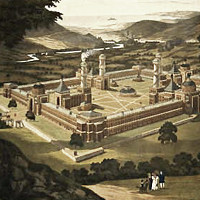
\includegraphics{../media/tbd_city01.jpg}   \end{wrapfigure} 

The houses there are wealthier, with influences from the far eastern cities of Asinalia, denoting a strong taste for delicate yet powerful ornaments. 

Such dedications for inspirating motives makes me cheerful, helping me to forget my spiritual loneliness.
The sun is beginning to annihilate the moisty effects of the mist, casting some orange lights on the walls.

What can I do now? 

\begin{gbitemize}
\gbitem Meet the local authorities, to announce myself and be registered: \textbf{\htmladdnormallink{44}{\#44}}
\gbitem Learn more about the customs and traditions: \textbf{\htmladdnormallink{33}{\#33}}
\gbitem Steal some goods, nobody knows me here after all: \textbf{\htmladdnormallink{40}{\#40}}
\end{gbitemize}

\hypertarget{26}{}
\pagebreak[\PAGExBREAKxPOLICY]
\textbf{\begin{center}\subsection*{\Huge{26}}\end{center}\vskip-2em}

\begin{itshape}

“Dear traveler,

thank you for being in my game. I hope you don't feel too restricted there, and your freedom of thoughts is not challenged. This short story may really begin when you'll arrived back into civilisation. Don't expect to discover much in those deserted islands. And if by chance you meet Jacqueline, say Hello to her.”

\end{itshape}

\begin{gbitemize}
\gbitem With some peace of mind and forgetting the luring greenness of the mountain, I row back to the boat: \textbf{\htmladdnormallink{11}{\#11}}
\end{gbitemize}

\hypertarget{27}{}
\pagebreak[\PAGExBREAKxPOLICY]
\textbf{\begin{center}\subsection*{\Huge{27}}\end{center}\vskip-2em}

The most notable thing in this place is a poster printed on an indigo background. Some big, pink letters are saying:

\begin{itshape}

“JOIN THE ARMY OF LOVE(TM)!

The Indigo Love Syndicate(tm) needs you. Thank you for your attention.”

\end{itshape}

There is no clear way to contact them. Probably they became so powerful recently that it's easy to find them. We'll see!

\begin{gbitemize}
\gbitem Tear the poster apart: \textbf{\htmladdnormallink{8}{\#8}}
\gbitem Pray in front of this colorful and appeasing poster: \textbf{\htmladdnormallink{36}{\#36}}
\gbitem Exit immediately: \textbf{\htmladdnormallink{25}{\#25}}
\end{gbitemize}

\hypertarget{28}{}
\pagebreak[\PAGExBREAKxPOLICY]
\textbf{\begin{center}\subsection*{\Huge{28}}\end{center}\vskip-2em}

I tell her about my philosophy of life, and the great goals everyone would like to achieve in the universe. I tell her about beauty, about the will, about ascetism and humility. 

Crying, the woman embrasses me, embarrassingly hanging to my neck, disowning her previous lovers.

\begin{gbitemize}
\gbitem Invite her to a teahouse, for talking more about important matters: \textbf{\htmladdnormallink{6}{\#6}}
\gbitem Leave her now, in order to increase her effervescency, and don't arrive too late at my home: \textbf{\htmladdnormallink{38}{\#38}}
\end{gbitemize}

\hypertarget{29}{}
\pagebreak[\PAGExBREAKxPOLICY]
\textbf{\begin{center}\subsection*{\Huge{29}}\end{center}\vskip-2em}

\setlength{\intextsep}{3mm} \begin{wrapfigure}{l}{0\textwidth} 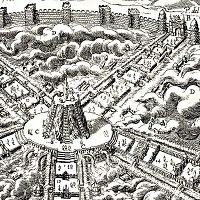
\includegraphics{../media/tbd_city02.jpg}   \end{wrapfigure} 

As soon as I enter the cyclopean building, I know this is the perfect place for me, a whole lifetime of commitment for serving literature, even with my approximative grammar and my Francimi accent.

\begin{center} THE END \end{center} 

\hypertarget{south}{}
\pagebreak[\PAGExBREAKxPOLICY]
\textbf{\begin{center}\subsection*{\Huge{30}}\end{center}\vskip-2em}

We head toward a strange island, a lone trail of yellow, backgrounded by green cliffs high above the beach. Once I arrive on the sand, I find a closed bottle on the ground. There is an old parchment inside.

\begin{gbitemize}
\gbitem Examine the bottle and its content: \textbf{\htmladdnormallink{26}{\#26}}
\gbitem Explore the island: \textbf{\htmladdnormallink{15}{\#15}}
\gbitem Go back to the boat: \textbf{\htmladdnormallink{11}{\#11}}
\end{gbitemize}

\hypertarget{31}{}
\pagebreak[\PAGExBREAKxPOLICY]
\textbf{\begin{center}\subsection*{\Huge{31}}\end{center}\vskip-2em}

Entering a brown cab carried by a Friesian horse, I quickly reach the small town where I live, in the suburb of the capital, and I stop at the cab station in the center. 

\begin{gbitemize}
\gbitem Should I really go strait home now: \textbf{\htmladdnormallink{38}{\#38}}
\gbitem or visit a friend of mine before that. I haven't seen her for a while, and we probably deserve to spend some good time together: \textbf{\htmladdnormallink{4}{\#4}}
\end{gbitemize}

\hypertarget{32}{}
\pagebreak[\PAGExBREAKxPOLICY]
\textbf{\begin{center}\subsection*{\Huge{32}}\end{center}\vskip-2em}

Someone sold me, while doing an important mission: I was supposed to meet an Indigo Love Syndicate leader, and capture him, but it was probably a trap, and \textbf{I} was captured instead.

\begin{gbitemize}
\gbitem Go to jail: \textbf{\htmladdnormallink{48}{\#48}}
\end{gbitemize}

\hypertarget{33}{}
\pagebreak[\PAGExBREAKxPOLICY]
\textbf{\begin{center}\subsection*{\Huge{33}}\end{center}\vskip-2em}

After a few researchs in the libraries and museum, I discover this society was founded one thousand years ago, after its physical separation from the Old Continent. It grew at a normal pace, without any noticeable events. More worrying is the fact that 10 years ago, a new sect, called the Indigo Love Syndicate, spread quickly across the continent, both among the populace and the elite. Discrete at the beginning, the sect is now one of the major political power in place.

\begin{gbitemize}
\gbitem I can join the opposition, to discover if they are better than what they pretend to fight: \textbf{\htmladdnormallink{9}{\#9}}
\gbitem I can forget about all those conspiracy stuffs, and lead a normal life, searching for a normal job: \textbf{\htmladdnormallink{52}{\#52}}
\end{gbitemize}

\hypertarget{34}{}
\pagebreak[\PAGExBREAKxPOLICY]
\textbf{\begin{center}\subsection*{\Huge{34}}\end{center}\vskip-2em}

During a sunny day, when most of the staff is with the family in holiday by the sea-side, I disable the electrical fences and climb the high walls, to reach liberty and self-realisation.

I forgot to get some goods with me, so I'm quite at loss in the streets, with my free will and my empty pockets.

\begin{gbitemize}
\gbitem Meet the local authorities, to be registered and begin a fair, remunerated, job: \textbf{\htmladdnormallink{47}{\#47}}
\gbitem Learn more about the customs and traditions: \textbf{\htmladdnormallink{33}{\#33}}
\gbitem Steal some foods and first necessity stuffs: \textbf{\htmladdnormallink{40}{\#40}}
\end{gbitemize}

\hypertarget{35}{}
\pagebreak[\PAGExBREAKxPOLICY]
\textbf{\begin{center}\subsection*{\Huge{35}}\end{center}\vskip-2em}

I compare her to a gorgeous and hot mare, to the goddess of fertility, war and lust, to the primeval nursemaid and such.

\begin{gbitemize}
\gbitem Strong as she is, I only get a well-deserved slap, and with the chin and cheek as red as an horny devil who ate pimento, and certainly ashamed, I go out in town: \textbf{\htmladdnormallink{41}{\#41}}
\end{gbitemize}

\hypertarget{36}{}
\pagebreak[\PAGExBREAKxPOLICY]
\textbf{\begin{center}\subsection*{\Huge{36}}\end{center}\vskip-2em}

\textit{Lorem ipsum dolor sit amet, consectetur adipisicing elit, sed do eiusmod tempor incididunt ut labore et dolore magna aliqua. Ut enim ad minim veniam, quis nostrud exercitation ullamco laboris nisi ut aliquip ex ea commodo consequat. Duis aute irure dolor in reprehenderit in voluptate velit esse cillum dolore eu fugiat nulla pariatur. Excepteur sint occaecat cupidatat non proident, sunt in culpa qui officia deserunt mollit anim id est laborum.}

I pray in collusion with all the followers of the Indigo Love Syndicate. 

I fell that my soul is somehow tainted now.

\begin{gbitemize}
\gbitem I continue nevertheless into the town: \textbf{\htmladdnormallink{22}{\#22}}
\end{gbitemize}

\hypertarget{37}{}
\pagebreak[\PAGExBREAKxPOLICY]
\textbf{\begin{center}\subsection*{\Huge{37}}\end{center}\vskip-2em}

Thinking probably I misunderstood her idle activity, the woman seems upset to be disturbed by my approach. She tells me frankly she's waiting for someone else and don't care about my disgraceful existance.

\begin{gbitemize}
\gbitem Insist more: \textbf{\htmladdnormallink{28}{\#28}}
\gbitem Insult her : \textbf{\htmladdnormallink{46}{\#46}}
\gbitem Come back home: \textbf{\htmladdnormallink{31}{\#31}}
\end{gbitemize}

\hypertarget{38}{}
\pagebreak[\PAGExBREAKxPOLICY]
\textbf{\begin{center}\subsection*{\Huge{38}}\end{center}\vskip-2em}

My appartment is in an almost deserted house with three floors. I live in the last floor, so I can see the woods from my bathroom. There is a huge forest in the eastern part of the town, where people can go hunting, hiking and ressourcing themselves from the modern way of life.

I feel so tired, that I go to bed immediately.

\begin{gbitemize}
\gbitem Wake up to \textbf{\htmladdnormallink{55}{\#55}}
\end{gbitemize}

\hypertarget{39}{}
\pagebreak[\PAGExBREAKxPOLICY]
\textbf{\begin{center}\subsection*{\Huge{39}}\end{center}\vskip-2em}

After being knocked down by a pirate with putrid teeth, I'm led to their lair, which is hidden in a big city I've never been before. Could it be I'm on the new Continent after all~?

I was separated from the other sailors to avoid rebellion, and met people with langage and culture I couldn't understand at all.

\begin{gbitemize}
\gbitem I hear the pirates are planning to sell me as a slave: \textbf{\htmladdnormallink{16}{\#16}}
\end{gbitemize}

\hypertarget{40}{}
\pagebreak[\PAGExBREAKxPOLICY]
\textbf{\begin{center}\subsection*{\Huge{40}}\end{center}\vskip-2em}

Stealing is easy here: it seems nobody is on guard so I can lure many people. In fact I didn't know the citizen weren't aware of misdeeds just because the police was so effective that criminals were caught within 48 hours.

\begin{gbitemize}
\gbitem Go to jail: \textbf{\htmladdnormallink{48}{\#48}}
\end{gbitemize}

\hypertarget{41}{}
\pagebreak[\PAGExBREAKxPOLICY]
\textbf{\begin{center}\subsection*{\Huge{41}}\end{center}\vskip-2em}

My sinful mood entangling my mind into so a well-known depression, I'm wandering in town without purpose. I'm crossing an ornamented iron bridge. A lamplighter is bringing light to the streets, without a smile. The dusk is leaving, replaced soon by the full night. The indigo sky is matching the indigo river and I'm longing for such an harmony.

\begin{itshape}Am I lucky today? When I get a die out of my pocket, I can be considered lucky when I cast a 5 or 6.\end{itshape}

\begin{gbitemize}
\gbitem If I'm lucky: \textbf{\htmladdnormallink{12}{\#12}}
\gbitem If I'm not lucky: \textbf{\htmladdnormallink{17}{\#17}}
\end{gbitemize}

\hypertarget{42}{}
\pagebreak[\PAGExBREAKxPOLICY]
\textbf{\begin{center}\subsection*{\Huge{42}}\end{center}\vskip-2em}

Beatrix' appartment is cozy and modern: lots of wooden furniture, ornamented with copper. She begins to remove her clothes, then think again and tells me she prefer we have a drink in a tavern.

\begin{gbitemize}
\gbitem Go out again, to find a tavern: \textbf{\htmladdnormallink{7}{\#7}}
\end{gbitemize}

\hypertarget{west}{}
\pagebreak[\PAGExBREAKxPOLICY]
\textbf{\begin{center}\subsection*{\Huge{43}}\end{center}\vskip-2em}

The western side of the sea is famous for its tricky tornados and whirlpools.
The destiny of our boat is yet challenged by some humanly disaster, when a pirate ship is attacking us.

The ruffians arrive on board, full of hate and violence, and even if we try to rebel, we're not strong enough to contain their assault for very long.

\begin{itshape}Am I lucky today? When I get a die out of my pocket, I can be considered lucky when I cast a 5 or 6.\end{itshape}

\begin{gbitemize}
\gbitem If I'm lucky: \textbf{\htmladdnormallink{39}{\#39}}
\gbitem If I'm not lucky: \textbf{\htmladdnormallink{54}{\#54}}
\end{gbitemize}

\hypertarget{44}{}
\pagebreak[\PAGExBREAKxPOLICY]
\textbf{\begin{center}\subsection*{\Huge{44}}\end{center}\vskip-2em}

They welcome me with great attention, and take my name. They note my request, and give me the number of an office on the second floor. 

\begin{itshape}Am I lucky today? When I get a die out of my pocket, I can be considered lucky when I cast a 5 or 6.\end{itshape}

\begin{gbitemize}
\gbitem If I'm lucky: \textbf{\htmladdnormallink{52}{\#52}}
\gbitem If I'm not lucky: \textbf{\htmladdnormallink{20}{\#20}}
\end{gbitemize}

\hypertarget{45}{}
\pagebreak[\PAGExBREAKxPOLICY]
\textbf{\begin{center}\subsection*{\Huge{45}}\end{center}\vskip-2em}

Mr and Mrs Caesar own a house which is bigger than anything I had already seen: a private aircraft landing place, a tower in the garden, electricity everywhere, for growing plants and vegetables...

They take me to their workshop, where I'm supposed to assembly stuffs and repair all the gadgets they have in the house: mecanical birds, electrical machines, phonographs...

After one year here, they begin to trust me.

\begin{gbitemize}
\gbitem will I try to escape when they are less watchful: \textbf{\htmladdnormallink{34}{\#34}}
\gbitem or continue to live here as a cheap laborer: \textbf{\htmladdnormallink{48}{\#48}}
\end{gbitemize}

\hypertarget{46}{}
\pagebreak[\PAGExBREAKxPOLICY]
\textbf{\begin{center}\subsection*{\Huge{46}}\end{center}\vskip-2em}

Coming from a dark corner, a man dressed in black hits me on the back.

\begin{gbitemize}
\gbitem I can see a blue veil covering my eyes: \textbf{\htmladdnormallink{14}{\#14}}
\end{gbitemize}

\hypertarget{47}{}
\pagebreak[\PAGExBREAKxPOLICY]
\textbf{\begin{center}\subsection*{\Huge{47}}\end{center}\vskip-2em}

They welcome me with great attention, and while taking my name, they show me a list of jobs in the surroundings.
I'm probably lucky, because there was recently a vacant place as a librarian in the main library.

After making me sign a few papers, they show me the road on a map.

\begin{gbitemize}
\gbitem Go there right now, in case somebody takes the place before me: \textbf{\htmladdnormallink{2}{\#2}}
\gbitem Learn more about the customs and traditions: \textbf{\htmladdnormallink{33}{\#33}}
\end{gbitemize}

\hypertarget{48}{}
\pagebreak[\PAGExBREAKxPOLICY]
\textbf{\begin{center}\subsection*{\Huge{48}}\end{center}\vskip-2em}

After a few years as a prisoner, I am more reasonnable, and seek redemption when I'm free again. Probably the best for me is to travel back home, and begin a new life there. Will I be librarian, or adventurer there? I still can't decide.

\begin{center} THE END \end{center} 

\hypertarget{49}{}
\pagebreak[\PAGExBREAKxPOLICY]
\textbf{\begin{center}\subsection*{\Huge{49}}\end{center}\vskip-2em}

During a mission, I don't feel I get the support I usually deserve, and I feel like I'm entering a trap, without any way out.

\begin{gbitemize}
\gbitem Enter the trap: \textbf{\htmladdnormallink{51}{\#51}}
\end{gbitemize}

\hypertarget{50}{}
\pagebreak[\PAGExBREAKxPOLICY]
\textbf{\begin{center}\subsection*{\Huge{50}}\end{center}\vskip-2em}

I tell her about my philosophy of life, and the great goals everyone would like to achieve in the universe. I tell her about beauty, about the will, about ascetism and humility. 

\begin{gbitemize}
\gbitem The woman have mercy, and with a perplexed smile, she leads me back to \textbf{\htmladdnormallink{44}{\#44}}
\end{gbitemize}

\hypertarget{51}{}
\pagebreak[\PAGExBREAKxPOLICY]
\textbf{\begin{center}\subsection*{\Huge{51}}\end{center}\vskip-2em}

An Indigo Love Cultist, jumping from a dark corner, is showing me some attention and dedication by stabbing my back.

\begin{gbitemize}
\gbitem I can see a blue veil covering my eyes: \textbf{\htmladdnormallink{14}{\#14}}
\end{gbitemize}

\hypertarget{52}{}
\pagebreak[\PAGExBREAKxPOLICY]
\textbf{\begin{center}\subsection*{\Huge{52}}\end{center}\vskip-2em}

In the office, they show me a list of jobs in the surroundings.
I'm probably lucky, because there was recently a vacant place as a librarian in the main library.

After making me sign a few papers, they show me the road on a map.

\begin{gbitemize}
\gbitem Go there right now, in case somebody takes the place before me: \textbf{\htmladdnormallink{29}{\#29}}
\gbitem Learn more about the customs and traditions: \textbf{\htmladdnormallink{33}{\#33}}
\end{gbitemize}

\hypertarget{53}{}
\pagebreak[\PAGExBREAKxPOLICY]
\textbf{\begin{center}\subsection*{\Huge{53}}\end{center}\vskip-2em}

A kind woman explains me with a soft voice the office I'm looking for is now on the first floor.

\begin{gbitemize}
\gbitem Which is leading to \textbf{\htmladdnormallink{44}{\#44}}
\gbitem Before that, I can try to seduce her by chance: \textbf{\htmladdnormallink{50}{\#50}}
\end{gbitemize}

\hypertarget{54}{}
\pagebreak[\PAGExBREAKxPOLICY]
\textbf{\begin{center}\subsection*{\Huge{54}}\end{center}\vskip-2em}

During the attack, I see the flashing blue of a pirate's sword, approaching my head so dangerously that I eventually die.

\begin{gbitemize}
\gbitem Go to \textbf{\htmladdnormallink{14}{\#14}}
\end{gbitemize}

\hypertarget{55}{}
\pagebreak[\PAGExBREAKxPOLICY]
\textbf{\begin{center}\subsection*{\Huge{55}}\end{center}\vskip-2em}

Yawning and stretching, I awake with a good mood. I haven't discovered a new Continent, I haven't experienced great adventures, but I met some people who weren't bad at all.

Day after day, I meet my friend Beatrix more and more often, and she tries to cope with my grim humor. She always tells me our story is really like an happy end after all!

\begin{center} THE END \end{center} 

% LaTeX2e code generated by txt2tags 2.6.804 (http://txt2tags.org)
% cmdline: txt2tags -T ..//templates/gamebook.tex --config-file ..//core/txt2cyoa.t2t -t tex --no-toc --outfile the_blue_death.tex the_blue_death.t2t

\end{LARGE}
\end{document}
